\documentclass[11pt,dvipdfm]{article}

\usepackage{deauthor,times,graphicx,listings}
%\usepackage[utf8]{inputenc}
%\usepackage[dvipdfm]{hyperref}
% \usepackage{xcolor}
 
%\graphicspath{{alonso/}}

%for table heades ro be centered
\newcommand{\centercell}[1]{\multicolumn{1}{c|}{#1}}
\newcommand{\head}[1]{\centercell{\textbf{#1}}}
\newcommand{\headlast}[1]{\multicolumn{1}{c}{\textbf{#1}}}

\newcommand{\dbname}{doppioDB}

\begin{document}
\title{doppioDB 1.0: Machine Learning inside a Relational Engine}
\author{Gustavo Alonso\(^1\), Zsolt Istvan\(^2\), Kaan Kara\(^1\), Muhsen Owaida\(^1\), David Sidler\(^1\) \\
\(^1\)Systems Group, Dept. of Computer Science, ETH Zurich, Switzerland \\
\(^2\)IMDEA Software Institute, Madrid, Spain }
% \date{May 2019}

\maketitle

\begin{abstract}
   Advances in hardware are a challenge but also a new opportunity. In particular, devices like FPGAs and GPUs are a chance to extend and customize relational engines with new operations that would be difficult to support otherwise. Doing so would offer database users the possibility of conducting, e.g., complete data analyses involving machine learning inside the database instead of having to take the data out, process it in a different platform, and then store the results back in the database as it is often done today. In this paper we present doppioDB 1.0, an FPGA-enabled database engine incorporating FPGA-based machine learning operators into a main memory, columnar DBMS (MonetDB). This first version of doppioDB provides a platform for extending traditional relational processing with customizable hardware to support stochastic gradient descent and decision tree ensembles. Using these operators, we show examples of how they could be included into SQL and embedded as part of conventional components of a relational database engine. While these results are still a preliminary, exploratory step, they illustrate the challenges to be tackled and the advantages of using hardware accelerators as a way to extend database functionality in a non-disruptive manner. 
\end{abstract}

% \newpage

 \section{Introduction}
Data intensive applications are often dominated by online analytic processing (OLAP) and machine learning (ML) workloads. Thus, it is important to extend the role of the database management system to a more comprehensive platform supporting complex and computationally intensive data processing. This aspiration is, however, at odds with existing engine architectures and data models. In this work, we propose to take advantage of the ongoing changes in hardware to extend database functionality without having to completely redesign the relational engine. The underlying hardware for this work, field programmable gate arrays (FPGAs), is becoming more common both in cloud deployments (e.g., Microsoft's Catapult or Amazon's F1 instances) and in conventional processors (e.g., Intel's hybrid architectures incorporating an FPGA into a CPU). FPGAs can be easily reprogrammed to provide the equivalent of a customizable hardware architecture. Thus, the FPGA can be used as a hardware extension to the database engine where additional functionality is implemented as a complement to that already available. 

We have implemented this idea in a first prototype of doppioDB, identified here as doppioDB 1.0 to distinguish it from future versions, showing how to integrate machine learning operators into the database engine in a way that is both efficient (i.e., compute-intensive algorithms do not impose overhead on native database workloads) and effective (i.e., standard operator models and execution patterns do not need to be modified). doppioDB runs on top of Intel's second generation Xeon+FPGA machine and it is based on MonetDB, an open source main memory columnar database.

 Combining machine learning (ML) tasks with database management systems (DBMS) is an active research field and there have been many efforts exploring this both in research \cite{hellerstein2012madlib, passing2017sql, aref2015design, cai2013simulation, mahajan2018rdbms} and industry ~\cite{farber2012sap,Tamayo2005}. This combination is attractive because businesses have massive amounts of data in their existing DBMS and there is a high potential for using ML to extract valuable information from it. In addition, the rich relational operators provided by the DBMS can be used conveniently to denormalize a complex schema for the purposes of ML tasks~\cite{wisconsinJoins2015}. 

 
%In fact, there a is growing amount of literature showing the potential of such an approach~\cite{casper2014hardware,jun2015bluedbm,sukhwani2012,woods2014ibex,salami2017axledb,woods2013fccm,sidler2017regex,kara2017fpga}. 



%The methods we use for integrating FPGA-based operators in doppioDB depart from previous approaches where the hardware acceleration is either located between the storage/network and the CPU where it is used mostly for predicate evaluation~\cite{woods2014ibex}, or on a dedicated system built from scratch to natively support hardware acceleration~\cite{mapd}. With doppioDB, we demonstrate that it is feasible and beneficial to integrate  emerging workloads by creating hardware accelerated SQL constructs to handle machine-learning operations such as Decision Trees and Stochastic Gradient Descent directly over relational data. 


\section{Prototyping Platform}
\label{sec:prototype-platform}
\subsection{Background on FPGAs}

Field Programmable Gate Arrays (FPGAs) are reconfigurable hardware chips. Once configured, they behave as application-specific integrated circuits (ASIC). Internally they are composed of programmable logic blocks and a collection of small on-chip memories (BRAM) and simple arithmetic units (DSPs)~\cite{jensFPGABook}. Their computational model is different from CPUs: instead of processing instruction by instruction, algorithms are laid out spatially on the device, with different operations all performed in parallel. Due to the close proximity of logic and memory on the FPGA, building pipelines is easy, and thanks to the flexibility of the on-chip memory, custom scratch-pad memories or data structure stores can be created.

Current FPGA designs usually run at clock-rates around 200-400\,MHz. To be competitive with a CPU, algorithms have to be redesigned to take advantage of deep pipelines and spatial parallelism. 
%As we show in this paper, this execution model fits well with column stores, but even if the processing model is more iterative, as in machine learning algorithms, the specialized hardware can offer significant benefits over software. 

%Once seen as highly specialized devices for digital design, today FPGAs have become an accepted hardware accelerator in many platforms~\cite{putnam2014reconfigurable, gupta2011harp}.



\subsection{Intel Xeon+FPGA Platform}
\label{sec:harp2}

While the use of FPGAs for accelerating data processing has been studied in the past, it is the emergence of hybrid CPU+FPGA architectures that enables their use in the context of a database with a similar overhead as NUMA architectures. In the past, FPGAs and other hardware accelerators, such as GPUs, have been placed ``on the side'' of existing database architectures much like an attachment rather than a component~\cite{ross2015gpu,netezza,jun2015bluedbm}. This approach requires data to be moved from the main processing unit to a detached accelerator. As a result, system designs where whole operators (or operator sub-trees) are offloaded to the accelerator are favored compared to finer integration of the accelerated operators into the query plan. We have designed doppioDB for emerging heterogeneous platforms where the FPGA has direct access to the main memory of the CPU, avoiding data copy. These platforms have also opened up opportunities of accelerating parts of operators such as partitioning or hashing~\cite{kara2017fpga} instead of full operations or even entire queries.

We use the second generation Intel Xeon+FPGA machine\footnote{Results in this publication were generated using pre-production hardware and software donated to us by Intel, and may not reflect the performance of production or future systems.}(Figure \ref{fig:harp-centaur}) that is equipped with an Intel Xeon Broadwell E5 with 14 cores running at 2.4\,GHz and, in the same package as the Xeon, an Intel Arria 10 FPGA. 
The machine has 64\,GB of main memory shared with the FPGA. Communication happens over 1\,QPI and 2\,PCIe links to the memory controller of the CPU. These are physical links as the FPGA is not connected via the PCIe bus. The resulting aggregated peak bandwidth is 20\,GB/s.

\begin{figure}[t]
    \begin{center}
        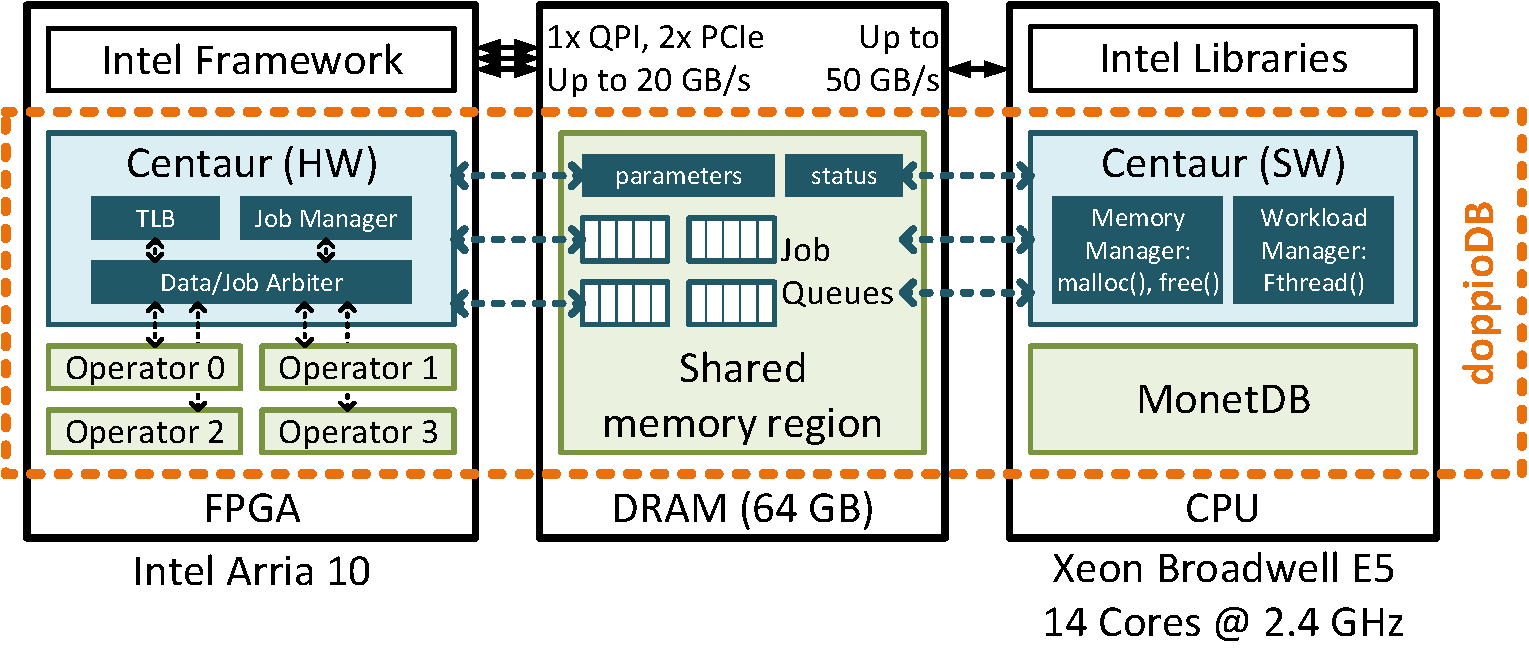
\includegraphics[width=0.8\textwidth]{figs/doppioDB.eps}
    \end{center}
\vspace{-2em}
	\caption{\dbname{} using Centaur on Intel's Xeon+FPGA second generation prototype machine.}
	\label{fig:harp-centaur}
\end{figure}

On the software side, Intel's {\em Accelerator Abstraction Layer} (AAL) provides a memory allocator to allocate memory space shareable between the FPGA and the CPU. %We were able to allocate up to 56\,GB out the available 64\,GB of main memory. 
This allows data to be accessed from both the CPU and the FPGA. Apart from the restrictions of the operating system, such as not supporting memory mapped files for use in the FPGA, the rest of the memory management infrastructure has remained untouched.

%\zsolt{put this in perspective of the memory allocator/workloads?}
%The AAL uses 2\,MB super pages as well as 4\,KB pages to allocate the shared memory space. The allocated pages are pinned to avoid page faults. The TLB on the FPGA has a configurable fixed size, 512 entries in our case, and can handle TLB misses.

%\begin{figure}[t]
%	\centering
%	\includegraphics[width=0.95\linewidth]{figures/harp-highlevel.png}
%	\caption{High level view of our prototype platform and software/hardware components running on it.}
%	\label{fig:harp2}
%\end{figure}

\subsection{MonetDB}
We use MonetDB as the basis of doppioDB.
MonetDB is an open source columnar read-optimized database designed for fast analytics. It stores relational tables as a collection of columns. A column consists of a memory heap with values and a non-materialized positional identifier. Because of this design, the values of a column are always stored in consecutive memory (or a memory mapped file) and they are addressable by simple memory pointers. MonetDB follows the operator-at-a-time paradigm and materializes the intermediate results of each operator. These design features make MonetDB suitable for integrating a hardware accelerator as they often require well-defined memory and execution boundaries per column and per operator.

%MonetDB's software stack comprises three layers: {\em 1)} the query language interface, {\em 2)} the server-side MAL intermediate representation (an assembly-like language), and {\em 3)} the GDK kernel. The first layer supports the parsing of the SQL language and the creation of the relational operator execution tree plan. In this layer many language specific optimizations take place, and also user defined functions (UDFs) are linked with the underlying implementation. The second layer of the MAL intermediate representation is responsible for orchestrating the query execution and apply system-specific optimizations. Finally, the 3rd layer, the GDK kernel, contains only foundational operators such as join and selections, as well as index creation and all memory allocation. This layered design is not unique to MonetDB, thus our efforts in doppioDB for integrating FPGAs to all three layers have applications beyond MonetDB.
%\section{Building a Customizable Database Engine}
%\label{sec:integration}
%\input{sections/integration}
%\subsection{Integration of Custom Hardware}

%One challenge of integrating specialized hardware in databases is that often the choice of what to offload is dictated by the way the accelerator is connected to the machine the database is running on (an on-the-side accelerator would for instance favor offloading compute-intensive operators, a smart storage engine would favor focusing on selection predicates for instance). With the emergence of shared-memory systems, such as the Intel Xeon+FPGA or IBM CAPI, the overhead of performing work on the specialized hardware has been reduced and this opens up acceleration opportunities across the stack. As a result, the choice of what to offload can be driven by the workloads and lead to overall better utilization of resources.
%In doppioDB we show that the underlying hardware device can be used to speed up operations across a wide spectrum: from the partitioning step of a join operator, through complex selection predicates, to stand-alone machine learning operations, such as model training. In doppioDB,we demonstrate that these can coexist in a single accelerator, and inside a single database engine. To achieve this, however, it requires two things: First, the customizable hardware needs to be exposed as part of the platform, with general purpose communication and management interfaces. Second, the functionality on the FPGA has to be designed in such a way that it fits inside the database engine without requiring data transformation or breaking encapsulation principles. In the following we outline the framework we used for communication, than we shortly discuss the two ways we integrated hardware functionality into the database.


\section{doppioDB: Overview}\label{sec:vision}

Integrating machine learning operators in an OLAP-oriented database such as MonetDB requires to tackle several challenges. Many ML operators are iterative and scan the data multiple times. For example, to train a model on an input relation, the relation should be materialized before training starts. In a tuple-at-a-time execution model of the operator tree, every operator is invoked once per input tuple. As a result, iterative ML operators cannot fit in this execution model without changing the query execution engine. On the other hand, in an operator-at-a-time execution model, an operator processes all the input tuples at once before materializing its result and passing it to the next operator in the tree. In this execution model, the iterative nature of an ML operator is hidden inside the operator implementation and does not require to be exposed to the query execution engine. In addition, an operator-at-a-time execution model eliminates the cost of invoking the FPGA operator for every tuple. %So, we developed doppioDB on top of MonetDB because it employs the operator-at-a-time execution model.

Another challenge is the row-oriented data format required for ML operators. Column-oriented data fits OLAP workloads well but most ML algorithms work at tuple-level and therefore require row-oriented data. This puts databases in a difficult position: if data is stored in a row format, OLAP performance suffers. Keeping two copies of the data, one in each format, would introduce storage overhead and would significantly slow down updates. An alternative is to introduce a data transformation step to convert column-oriented data to a row-oriented format.
Transforming data on-the-fly using a CPU is possible, but leads to cache-pollution and takes away computation cycles from the actual algorithm. However, on the FPGA, the transformation step can be performed using extra FPGA logic and on-chip memory resources without degrading processing throughput or adding overhead on the query runtime as we discuss in Section~\ref{sec:gather-engine}. 

% \begin{figure}[t]
%    \centering
%    \includegraphics[width=0.8\textwidth]{figs/STOCK.eps}
%    \caption{An example schema showing a selective denormalization and model training using SGD.}
%    \label{fig:stock}
%\end{figure} 

% \begin{figure}[t]
% 	\includegraphics[width=\columnwidth]{figures/STOCK.png}
% 	\caption{An example schema showing a selective denormalization and model training using SGD.}
% 	\label{fig:stock}
% \end{figure}

When adding new functionality to the database engine, a constant challenge is how to expose this functionality at the SQL level. The use of user defined functions (UDFs) is a common practice, but there are some significant drawbacks with this approach. First, UDFs limit the scope of applicability of the operator, e.g., they do not support updates or they are applied to one tuple at a time. Second, usually a query optimizer perceives UDFs as black boxes that are pinned down in the query plan, missing optimization opportunities. We believe extending SQL with new constructs and keywords allows a better exposure of the functionality and the applicability of complex operators. However, this is not easy to achieve, since the order of execution and the rules of the SQL language has to be respected. Later in the paper we discuss different SQL extensions for ML operators.

%Although at first glance the combination looks like it benefits both DBMS and ML, a major drawback is the potential performance impact on query processing when compute intensive and inherently iterative ML tasks run on the same processor as traditional SQL queries. As we show in this work, when using the FPGA to run a compute-intensive task, doppioDB's performance for software queries is almost unchanged, which shows that hardware-based methods offer good performance isolation between different types of queries.
%One of our objectives through this work is to demonstrate the extensibility of doppioDB through using open-source implementations of different operators. we show that minimal 
%\paragraph{\textbf{Design overview}}
%doppioDB uses hardware to speed up operations across a wide spectrum: from the partitioning step of a join operator, through complex selection predicates, to stand-alone machine learning operations, such as model training. Furthermore these can coexist in a single accelerator, inside a single database engine. 

Since FPGAs are not conventional compute devices, there is no general software interface for FPGA accelerators. Typically, every accelerator has its own software interface designed for its purposes. However, in the database environment where many different operators will use the FPGA, the customizable hardware needs to be exposed as part of the platform, with general purpose communication and management interfaces. We have implemented the communication between MonetDB and the FPGA using the open-source Centaur\footnote{\url{https://github.com/fpgasystems/Centaur}}~\cite{owaida-fccm2017} framework, which we modify to provide better memory access and extend with a data transformation unit that can be used by operators that require a row-oriented format instead of the default columnar format of MonetDB. 


\section{Database integration of FPGA based operators}
\label{sec:HAL}

\subsection{Communication with the FPGA}
\label{sec:centaur}

There have been many efforts in the FPGA community to generalize FPGA accelerators through software abstractions and OS-like services for CPU-FPGA communication. Examples of these efforts include hThreads~\cite{andrews2004hybridthreads}, ReconOS~\cite{lubbers2009reconos}, and Centaur~\cite{owaida-fccm2017}. Since Centaur is developed for the Intel Xeon+FPGA prototype machine and it is open source, we decided to use it in developing doppioDB. 
%We use Centaur, an open-source framework, for integrating FPGA accelerators into software applications, developed by Owaida et. al~\cite{owaida-fccm2017} for the first generation Intel Xeon+FPGA prototype machine. 
In this work, we port Centaur to Intel's second generation Xeon+FPGA (Broadwell+Arria10) platform.

% What it is: its objective, what facilitates
Centaur abstracts FPGA accelerators as hardware threads and provides a clean thread-like software interface, called \emph{FThread}, that hides the low level communication between FPGA and CPU. Its \emph{Workload Manager} (Figure~\ref{fig:harp-centaur}) allows for concurrent access to different operators. It guarantees concurrency by allocating different synchronous job queues for different operators types. Overall, this makes it possible to share FPGA resources between multiple queries and database clients. Centaur's \emph{FThread} abstraction allows us to express FPGA operators as separate threads which can be invoked from anywhere in doppioDB. For example, we can use data partitioning on the FPGA as shown in Listing~\ref{centaur_op}. We create an \emph{FThread} specifying that we want to perform partitioning on relation R with the necessary configuration, such as the source and destination pointers, partitioning fanout, etc. After the \emph{FThread} is created, the parent thread can perform other tasks and finally the \emph{FThread} can be joined to the parent similar to C++ threads.



By creating the \emph{FThread} object, we communicate a request to the FPGA to execute an operator. Internally, the request is first queued in the right concurrent job queue allocated in the CPU-FPGA shared memory region, as shown in Figure~\ref{fig:harp-centaur}. Then, Centaur's \emph{Job Manager} on the FPGA, monitoring the queues continuously, dequeues the request and starts the execution of the operator. In case all operators of the requested type are already allocated on the FPGA by previous requests, the \emph{Job Manager} has to wait until an operator becomes free before dispatching the new request. The Job Manager scans the different job queues in the shared memory concurrently and independent of each other such that a job queue that has free operator is not blocked with another queue waiting on a busy operator.

On the FPGA, Centaur partitions the FPGA into four independent regions each hosting an accelerator (examples shown in Figure~\ref{fig:harp-centaur}). Centaur's \emph{Job Manager} facilitates CPU-FPGA communication and enables concurrent access to all accelerators. In addition, the \emph{Data Arbiter} multiplexes the access to the memory interface from multiple operators using a round-robin mechanism. 

\begin{lstlisting}[float=tp,frame=single,breaklines=true,language=C++, basicstyle=\footnotesize, label=centaur_op,caption=An FPGA operator representation in Centaur., keywords={FThread, join}]
relation *R, *partitioned_R;
...
// Create FPGA Job Config
PARTITIONER_CONFIG config_R;
config_R.source = R;
config_R.destination = partitioned_R;
config_R.fanout = 8192;
...
// Create FPGA Job
FThread R_fthread(PARTITIONER_OP_ID, config_R);
...
// Do some other work
...
// Wait for FThreads to finish
R_fthread.join();
...
\end{lstlisting}

% \begin{figure}[t]
% 	\centering
% 	\includegraphics[width=0.5\textwidth]{figs/CENTAUR.eps}
% 	\caption{Centaur on Intel's Xeon+FPGA second generation prototype machine.}
% 	\label{fig:centaur}
% \end{figure}

\paragraph{\textbf{Porting Centaur to the target platform.}} Centaur's \emph{Memory Manager} implements a memory allocator that manages the CPU-FPGA shared memory region. However, we discovered through our experiments that this custom memory allocator incurs a significant overhead in certain workloads. This is mostly due to a single memory manager having to serve a multi-threaded application from a single memory region. To overcome this, we allow the database engine to allocate tables in the non-shared memory region using the more sophisticated operating system memory allocation. Then, we perform memory copies from the non-shared to the shared memory region only for columns used by the FPGA operators. This is not a fundamental requirement and is only caused by the limitations of the current FPGA abstraction software stack: In future iterations of the Xeon+FPGA machine, we expect that the memory management for FPGA abstraction libraries will be integrated into the operating system, thus giving Centaur the ability to use the operating system memory allocation directly. The FPGA can then access the full memory space, without memory copies.

Beyond the modification to the memory allocator, we changed the following in Centaur: First, we clocked up Centaur FPGA architecture from 200\,MHz to 400\,MHz to achieve a 25\,GB/s memory bandwidth. Operators can still be clocked at 400 or 200\,MHz. 
In addition, we replaced the FPGA pagetable, which is limited to 4 GB of shared memory space, with the Intel's MPF module which implements a translation look-aside buffer (TLB) on the FPGA to support unlimited shared memory space. We also added a column to row conversion unit to support operators which require row-oriented data format. 

%\paragraph{\textbf{Technical specifications.}} 

%In porting Centaur to our target platform, we had to perform several modifications. In the first version of the Intel's Xeon+FPGA platform, Centaur operates at 200 MHz, on the the target platform, we upgraded Centaur to operate at 400 MHz such that it reaches 25 GB/s memory bandwidth. However, the operators can be clocked at 400 or 200 MHz. 
%In addition, the first version of Centaur can allocate and manage up to 4 GB of virtual memory shared between the CPU and the FPGA, and the complete pagetable can be stored in the FPGA as it is relatively small. However, in our target platform, the FPGA has access to a much larger virtual memory region (up to 56 GB), storing the complete pagetable on the FPGA becomes wasteful in terms of on-chip memory resources. Hence, we replace Centaur's pagetable with Intel's MPF module, which implements a translation look-aside buffer (TLB) on the FPGA while keeping the much larger pagetable in main memory.

%Another improvement on the new Intel's Xeon+FPGA platform is the larger memory bandwidth available to the FPGA, 20 GB/s compared to 6 GB/s on the first prototype. Centaur clocked at 200 MHz, does not exploit fully the available memory bandwidth. We had to clock up Centaur's hardware circuits to 400 MHz to use the full memory bandwidth.  



\subsection{On-the-fly Data Transformation}
\label{sec:gather-engine}

In doppioDB we support machine learning operators on columnar data by adding a ``transformation'' engine that converts data on-the-fly to a row-oriented representation (Figure~\ref{fig:gather}). The engine is part of the \emph{Data Arbiter} in Figure~\ref{fig:harp-centaur} which is plugged in front of the operator logic. The design can be generalized and such transformations can be done across many different formats (data encodings, sampling, compression/decompression, encryption/decryption, summarization, etc.), a line of research we leave for future work. Such transformations are essentially "for free" (without impacting throughput and using a small part of the resources) in the FPGA   and, as such, will change the way we look at fixed schemas in database engines.

When designing this engine we made several assumptions. First, data belonging to each dimension resides in its own column, and the ordering of tuples per column is the same (there are no record-IDs, tuples are associated by order instead) . This allows us to scan the different columns based on a set of column pointers only. While the actual type of the data stored in each column is not important for this unit, our current implementation assumes a data width of 4\,Bytes per dimension. This is, however, not a fundamental limitation and the circuit could be extended to support, for instance, 8\,Byte values as well. 

\begin{figure}[t]
    \centering
	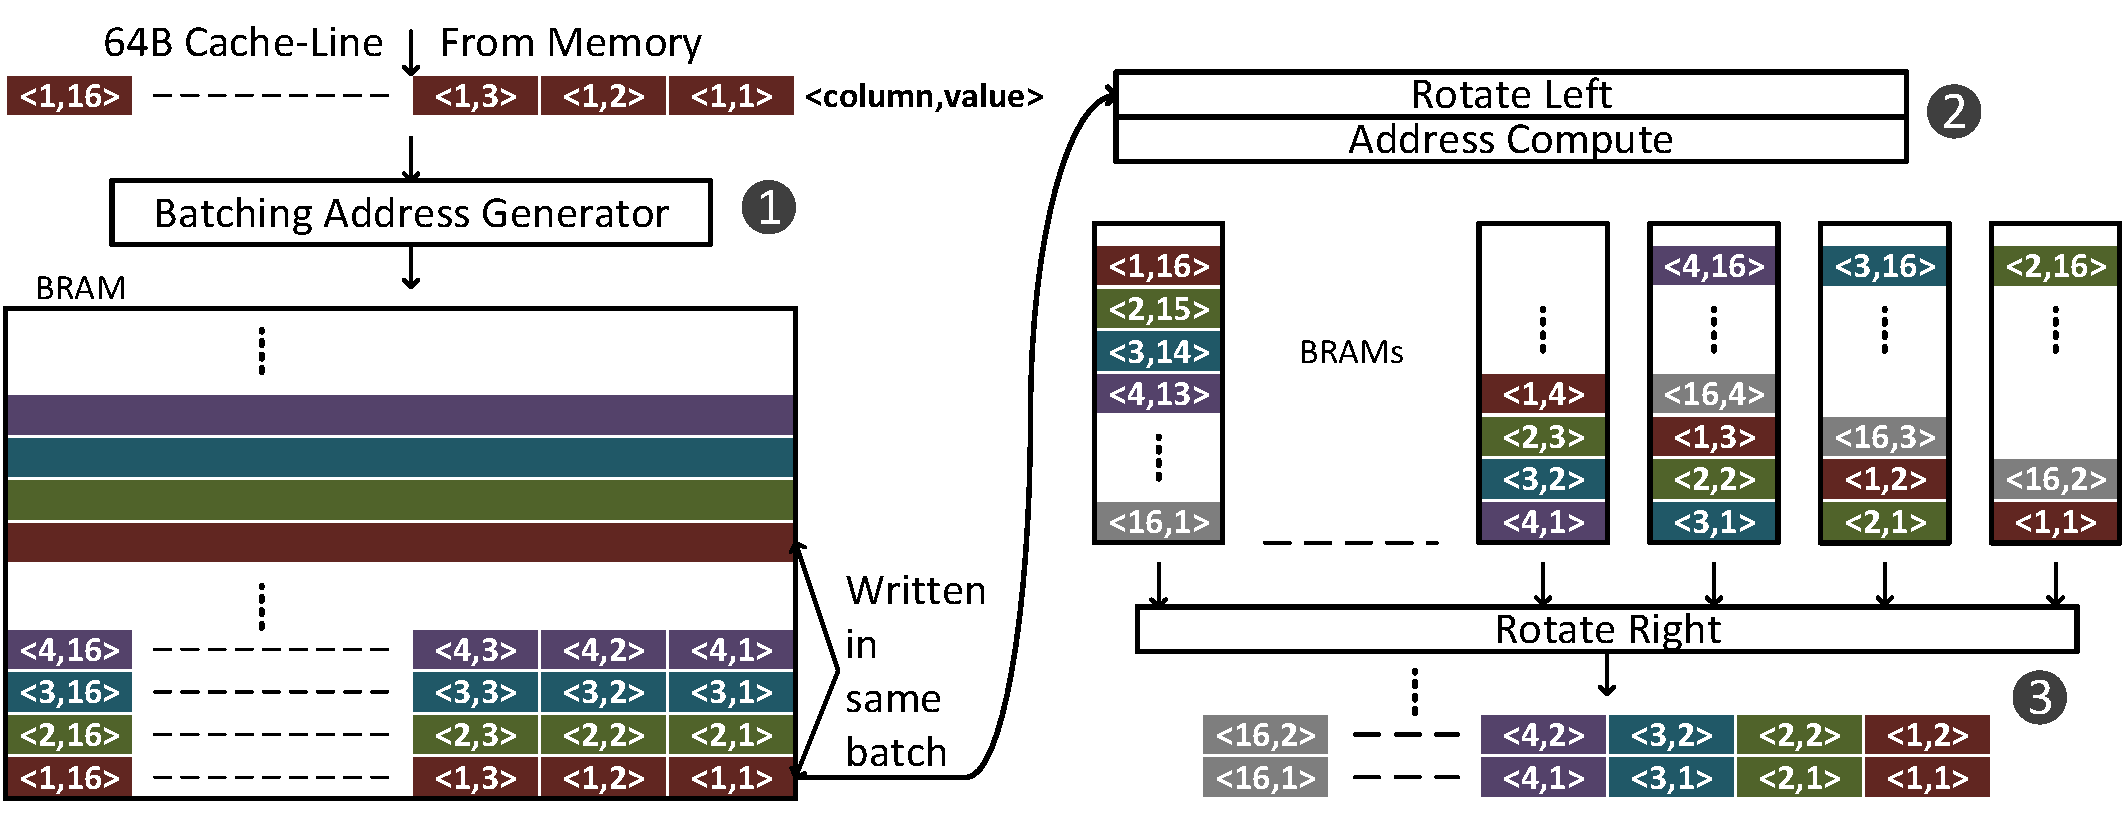
\includegraphics[width=0.8\textwidth]{figs/GATHER2.eps}
	\caption{On the FPGA the transformation from columns to rows can be implemented as a streaming operation that introduces latency but has constant bandwidth.}
	\label{fig:gather}
\end{figure}

The gather engine, as depicted in Figure \ref{fig:gather}, requests data belonging to different columns in batches to reach high memory bandwidth utilization. A batch is a number of successive cache lines requested from a single dimension column before reading from the next dimension column. Each cache line contains 16 entries of a column (16*4\,B=64\,B). The incoming data is scattered across a small reorder memory such that, when read sequentially, this memory returns one line per dimension (1). In the next step these lines are rotated and written into smaller memories in a ``diagonal'' fashion (2). This means that if the first 4 bytes are written to address 0 of the first memory, the second 4 bytes will go to address 1 of the second memory and so on. This layout ensures that when reading out the same address in each of these small memories, the output will contain one 4 Byte word from each dimension. With an additional rotate operation, we obtain a cache-line having values from each column in their respective positions (3). Thus, the flexibility of the FPGA allows us to build a ``specialized cache'' for this scatter-gather type of operation that would not be possible on a CPU's cache.

The nominal throughput of this unit is 12.8\,GB/s at 200 MHz and is independent of the number of dimensions. %To achieve this nominal throughput we use read-batching. %Our experiments showed that a minimum batching factor equals 32 is required to achieve maximum throughput. 
As Figure~\ref{fig:gatherthput} shows, throughput close to the theoretical maximum can already be achieved when batching 32 cache lines. The effect of having multiple dimensions is visible because DRAM access is scattered over a larger space, but with a sufficiently large batch size, all cases converge to 11.5\,GB/s.


\begin{figure}[t]
    \centering
    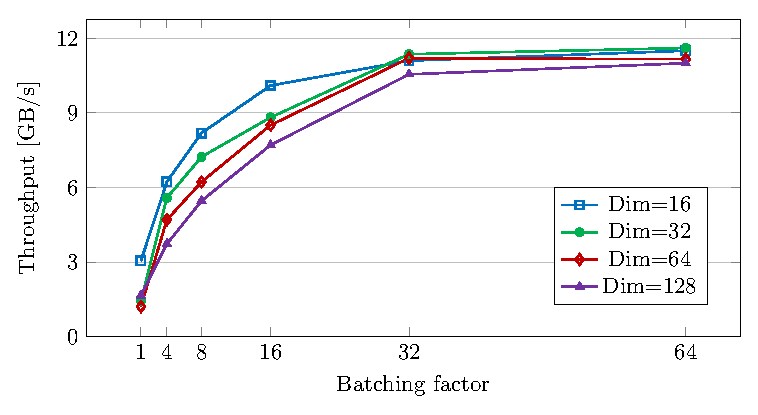
\includegraphics[width=0.7\textwidth]{figs/data-transformation-graph-crop.eps}
	\caption{Streaming transformation from columns to rows reaches high throughput and is not impacted negatively by the number of dimensions to be gathered.}
	\label{fig:gatherthput}
\end{figure}

%\begin{figure}[t]
%	\centering
% 	\begin{tikzpicture}
% 	\begin{axis}[
% 	legend style={at={(1.5,0.1)},
% 			anchor=south east, font=\small},
% 	width=0.75\columnwidth, height=0.45\columnwidth,
% 	ylabel=Throughput (GB/s),		
% 	xlabel=Batching factor,
% 	xtick={1, 4, 8, 16, 32, 64},
% 	xticklabels={1, 4, 8, 16, 32, 64},
% 	ymin=0,
% 	ytick={0,3,6,9,12},
% 	]
% 	\addplot [color=blue, mark=square, mark size=1.5]
% 	coordinates { (1,3.05) (4,6.23) (8,8.19) (16,10.1) (32,11.1) (64,11.5) };
% 	\addplot [color=green, mark=*]
% 	coordinates { (1,1.44) (4,5.58) (8,7.23) (16,8.82) (32,11.36) (64,11.61) };
% 	\addplot [color=red, mark=diamond]
% 	coordinates { (1,1.21) (4,4.7) (8,6.22) (16,8.51) (32,11.2) (64,11.16) };
% 	\addplot [color=brown, mark=triangle*]
% 	coordinates { (1,1.66) (4,3.73) (8,5.46) (16,7.71) (32,10.55) (64,11) };
	
% 	\legend{Dim=16, Dim=32, Dim=64, Dim=128} 
% 	\end{axis}
% 	\end{tikzpicture}
%	\caption{Streaming transformation from columns to rows reaches high throughput and is not impacted negatively by the number of dimensions to be gathered.}
%	\label{fig:gatherthput}
%\end{figure}

In terms of resource requirements, the number of BRAMs needed to compose the scatter memory depends on the maximum number of dimensions and the maximum batching factor, since at least one batch per dimension has to be stored. The choice for both parameters is made at compile-time. At runtime it is possible to use less dimensions and, in that case, the batching factor can be increased correspondingly. The number of the smaller memories is fixed (16), but their depth depends on the maximum number of dimensions. Even when configured for up to 256 dimensions with a batching factor of 4, only 128 kB %10\% 
of the on-chip BRAM resources are needed for this circuit. 


\section{Stochastic Gradient Descent}
\label{sec:sgd}
\paragraph{\textbf{Overview}}

By including a stochastic gradient descent (SGD) in doppioDB, our goal is to show that the FPGA-enabled database is capable of efficiently handling iterative model-training tasks. The SGD operator enables us to \textit{train} linear regression models and support vector machines (SVM) on the FPGA using relational data as input. There has been many studies showing the effectiveness of FPGA-based training algorithms~\cite{kesler2011hardware, bin2016fpgasvm, kara2017fpga2, mahajan2018rdbms, he2018flexible}. We based our design on open-sourced prior work by Kara et al.~\cite{kara2017fpga2}, which performs both gradient calculation and model update on the FPGA using fine grained parallelism and a pipelined design.
We integrated the SGD training algorithm into a DBMS in two steps: We extended SQL to enable a user's \textit{declarative} interaction with ML operators, followed by the physical integration of FPGA-accelerated ML operators into the DBMS.

\begin{lstlisting}[float=tp,frame=single,breaklines=true,language=sql,keywords={INSERT,INTO,SELECT,FROM,CREATE,MODEL,ON,USING,WITH,OVER,WHERE,INFER},caption=Template queries to train models on relations and do inference with trained models,basicstyle=\small,label={lst:MLsyntax}]
Q_train: CREATE MODEL model_name ON 
            (SELECT attr1, attr2, ..., label FROM data_set WHERE ...)
         WITH model_type USING training_algorithm(algorithm_parameters);

/*Infer without modifying the table*/
Q_infer1: SELECT new_data_set.id, 
          INFER('model_name') FROM new_data_set;

/*Infer and save results into a table*/
Q_infer2: INSERT INTO inferred_data_set(label)
          SELECT INFER('model_name') FROM new_data_set;
\end{lstlisting}

\paragraph{\textbf{SQL Integration}}
There has been many efforts to enable the usage of ML operators directly from SQL. While most efforts (MADlib \cite{hellerstein2012madlib}, SAP HANA~\cite{farber2012sap} and Oracle Data Miner~\cite{Tamayo2005}) expose ML operators as user defined functions (UDFs), some recent work considered extending SQL with new keywords to make ML operators in SQL more transparent. For instance, Passing et al.~\cite{passing2017sql} propose to introduce the "ITERATE" keyword to SQL to represent the iterative nature of ML training algorithms. To accomplish the same goal, Cai et al.~\cite{cai2013simulation} propose the "FOR EACH" keyword. In this work, we argue that the interaction with ML operators in a DBMS should be done in a more simple and intuitive way than previously proposed. To accomplish this, we propose a new SQL structure as shown in Listing~\ref{lst:MLsyntax}.

With the structure shown in Listing~\ref{lst:MLsyntax}, the user specifies (1) the model name after \textbf{CREATE MODEL}, (2) the attributes and the label that the model should be trained on after \textbf{ON}, (3) the type of the ML model after \textbf{WITH} (e.g., support vector machine, logistic regression, decision trees, neural networks etc.), (4) the training algorithm along with the parameters after \textbf{USING} (e.g., SGD, ADAM etc.). After the model is created, we can use it for inference on new tables using the \textbf{INFER} keyword, passing the model name. A model in doppioDB contains besides the actual ML model parameters also meta-parameters, specifying which attributes it was trained on. The \textbf{INFER} function ensures during query compilation that it receives all the attributes necessary according to the meta-parameters of the model. Otherwise, the SQL compiler raises a compile time error.

\begin{lstlisting}[float=tp,frame=single,breaklines=true,language=sql,keywords={SELECT,FROM,CREATE,MODEL,ON,USING,WITH,OVER,WHERE},caption=Queries to train various models on any desired projection using SGD. ,basicstyle=\small,label={lst:sgdquery}]
Q1: CREATE MODEL proteins_model ON 
       (SELECT attr1, attr2, ..., attr15, label FROM human_proteome)
    WITH LINREG USING SGD(num_iterations, learning_rate);

Q2: CREATE MODEL detect_fraud ON
       (SELECT Name, ..., IsFraud FROM transactions
       WHERE IsFraud IS NOT NULL)
    WITH SVM USING SGD(num_iterations, learning_rate);

Q3: CREATE MODEL stock_predictor ON
       (SELECT Region, ..., OpenCloseValues.Close FROM Transactions, Actors, Stocks, OpenCloseValues
       WHERE Stocks.Region = 'Europe' AND YEAR(OpenCloseValues.Date) > 2010 AND Actors.Position = 'Manager')
    WITH SVM USING SGD(num_iterations, learning_rate);
\end{lstlisting}

\begin{lstlisting}[float=tp,frame=single,breaklines=true,language=sql,keywords={SELECT,FROM,INFER,ON,WHERE,AS},caption=Inference queries to make predictions on tuples with empty labels.,basicstyle=\small,label={lst:inferquery}]
Q1: SELECT human_proteome.id, INFER('proteins_model') AS prediction 
    FROM human_proteome WHERE label IS NULL;

Q2: SELECT transactions.name, INFER('detect_fraud') 
    FROM transactions WHERE IsFraud IS NULL;

Q3: SELECT Stocks.Name, INFER('stock_predictor')
    FROM Transactions, Actors, Stocks, OpenCloseValues
    WHERE OpenCloseValues.Close IS NULL;
\end{lstlisting}

Listing~\ref{lst:sgdquery} shows how the syntax we introduce can be used on realistic scenarios. For instance, in \emph{Q3}, the ability to perform multiple joins and selections on four relations and then to apply a training algorithm on the projection is presented. This is a very prominent example showing the convenience of declarative machine learning. In Listing~\ref{lst:inferquery}, three inference queries with \textbf{INFER} are presented, using the models created by \textbf{CREATE MODEL} queries, again showing the convenience of performing prediction on tuples with an empty label.


\vspace{-.5em}

\paragraph{\textbf{Physical Integration}} The trained model is stored as an internal data structure specific to given relational attributes --similar to an index-- in the database. Inside the \textbf{CREATE MODEL} query, the training (iterative reading) happens over the resulting projection of the subquery inside \textbf{ON}(...). The operator-at-a-time execution of MonetDB fits well here: The training-related data is materialized once and is read multiple times by the SGD engine. In case of FPGA-based SGD, the pointers to the materialized data (multiple columns) are passed to the FPGA, along with training related parameters such as the number of iterations and the learning rate. The FPGA reads the columns corresponding to different attributes with the help of the gather engine as described in Section~\ref{sec:gather-engine}, reconstructing rows on-the-fly. The reconstruction is needed, because SGD requires all the attributes of a sample in the row-format to compute the gradient.

The tuples created by the subquery are read as many times as indicated by the number of iterations. For each received tuple, the SGD-engine computes a gradient using the model that resides on the FPGA-local on-chip memory. The gradient is directly applied back to the model on the FPGA, so the entire gradient descent happens using only the on-chip memory, reserving external memory access just for the training data input. After the training is complete, the model is copied from on-chip memory to the main memory of the CPU, where doppioDB can use it to perform inference.


\vspace{-.5em}

\paragraph{\textbf{Evaluation}}
We use the following data sets in our evaluation:
(1) A human proteome data set \cite{wilhelm2014mass}, consisting of 15 protein-related features and 38 Million tuples (Size: 2.5 GB); (2) A synthetic financial data set for fraud detection \cite{lopez2016paysim}, consisting of 6 training-related features and 6.4 Million tuples (Size: 150 MB); and (3) A stock exchange data set, consisting of 5 training-related features and 850 Thousand tuples (Size: 17 MB).

\begin{table}[t]
% 	\small
\vspace{-.5em}
	\centering
	\caption{Stochastic Gradient Descent Training Time}
\vspace{-.5em}
	\def\arraystretch{1.2}
	\begin{tabular}{l|r|r|r|r|r}
		\textbf{Data set} & \head{\#Tuples} & \head{\#Feat.} & \head{\#Epochs} & \head{doppioDB (CPU)} & \headlast{doppioDB (FPGA)} \\
		\hline
		\emph{proteome}     & 38\,Mio.   & 15 & 10  & 10.55\,s & 3.44\,s \\
		\emph{transactions} & 6.4\,Mio.  & 6  & 100 & 7.35\,s  & 2.54\,s \\
		\emph{stocks}       & 850\,K.    & 5  & 100 & 0.92\,s  & 0.32\,s \\
	\end{tabular} 
	%}
	\label{tab:sgd-result}
\end{table}

In Table~\ref{tab:sgd-result}, we present the time for training a linear SVM model on the data sets, using either the CPU or FPGA implementation. In both cases, the number of epochs (one epoch is defined as a full iteration over the whole data set) and learning rates are set to be equal. Therefore, the resulting models are statistically equal as well. Achieving multi-core parallelism for SGD is a difficult task because of the algorithm's iterative nature, especially for lower dimensional and dense learning tasks. Therefore, we are using a single-threaded and vectorized implementation for the CPU execution. We observe that the FPGA-based training is around 3x faster for both data sets, providing a clear performance advantage. The FPGA-based implementation~\cite{kara2017fpga2} offers finer grained parallelism, allowing the implementation of specialized vector instructions just for performing SGD, and also puts these instructions in a specialized pipeline, thereby providing higher performance. It is worth noting that the models we are training are linear SVM models, which are relatively small and on the lower compute intensive side compared to other ML models such as neural networks. For larger and more complex models, the performance advantage of specialized hardware will be more prominent~\cite{umuroglu2017finn, nurvitadhi2017can}. 




\section{Decision Tree Ensembles}
\label{sec:dt}

\vspace{-.5em}
\paragraph{\textbf{Overview}}
A \emph{decision tree} is a supervised machine learning method used in a wide range of classification and regression applications. %For example, one can train a decision tree on a financial data set to predict if an investment will be profitable or not. 
%Recently, decision tree ensembles (i.e., a collection of multiple trees) have become more popular than single trees, because of their higher accuracy.  
%Figure shows a decision tree example, and depicts how an input data record is processed to produce the classification result.  
 %A supervised machine learning algorithm consists of two steps: the training step where a training data set (which is already classified) is used to create the model. Then in the testing or \emph{inference} step, the model is used to classify new tuples. In this paper we only consider the inference step, where  the decision tree operator uses a stored model to classify the target tuples. 
%In the inference step, a tuple traverses the tree from the root node to a leaf node. At each level in the tree, an attribute of the tuple is compared against a tree node criteria to choose the right or left node in the next level. A leaf node stores the classification or regression result. In an ensemble, each tree is inferred independently, then the results of the individual trees are aggregated to produce the final classification or regression value.   
There have been a large body of research considering the use of FPGAs and accelerators to speedup decision tree ensemble-based inference~\cite{owaidafpl2017, owaidafpl2018,ObergFPL12,essenfccm12,yun2014}. The work of Owaida et al.~\cite{owaidafpl2017,owaidafpl2018} proposes an accelerator that is parameterizable at runtime to support different tree models. This flexibility is necessary in a database environment to allow queries using different models and relations to share the same accelerator. In doppioDB we base our FPGA decision tree operator on the design in~\cite{owaidafpl2017}.
%While the inference of a single decision tree is sequential in nature and memory bound, a large tree ensemble with tens of trees is compute bound. Accelerators in the form of FPGAs can 

%\paragraph{\textbf{Implementation}}
%In this paper, we base our FPGA decision tree operator on an implementation from Owaida et.al~\cite{} which parallelizes the inference of large tree ensembles. 
%explain the basic building block  
%The implementation resembles a many core architecture with custom processing elements (\emph{PE}) and dedicated circuitry for aggregating individual trees results as Figure~\ref{fig:dt-arch} shows. Each PE unit is capable of storing and processing multiple trees depending on the tree size. The PE unit data path implements the basic operations required to evaluate one level in the tree: read a tree node data structure, read a data record attribute, then compare the data attribute against the tree node criteria and determine the next level node. The PE data path iteratively applies these operations until all the tree level are evaluated. The data path pipelines the processing of multiple trees to hide the latency of evaluating a single tree and achieve high throughput. 
%The  dedicated aggregation circuitry collects all individual tree results and produce one value (floating point) per data record. 
%\begin{figure}[t]
%	\centering0930
%	\includegraphics[width=0.7\linewidth]{figures/monet-arch.png}
%	\caption{Decision tree FPGA operator architecture.}
%	\label{fig:dt-arch}
%\end{figure} 

%What we changed: use the gatherer module. 


\paragraph{\textbf{Integration in doppioDB}}

The original implementation works on row-oriented data, so as a first step, we replaced the data scan logic with the gather engine described in Section~\ref{sec:gather-engine}. As a result our implementation operates on columnar data in doppioDB without the need for any further changes to the processing logic. 
%how we represent a model in MonetDB, how we apply inference on inserted tuples. 
To integrate the decision trees into doppioDB, we use the same SQL extensions proposed for SGD to create models and perform inference as in Listing~\ref{lst:MLsyntax}. In Listing~\ref{lst:dtinfer} we show two examples of training and inference queries for the \emph{higgs} and \emph{physics} relations.
Since currently we do not implement decision tree training in doppioDB, the training function \emph{DTree('filename')} imports an already trained model from a file. The trained model can be obtained from any machine learning framework for decision trees such as XGBoost~\cite{chenkdd2016}. Inside doppioDB, the model is stored as a data structure containing information about the list of attributes used to train the model, the number of trees in the ensemble, the maximum tree depth, the assumed value of a missing attribute during training, and a vector of all the nodes and leaves of all the ensemble trees. 

The \textbf{INFER} function invokes the FPGA decision tree operator by passing the model parameters and pointers
to all the attribute columns to the FPGA. The FPGA engine then loads the model and stores it in the FPGA local memories. Then, the gather engine scans all the attribute columns and constructs tuples to be processed by the inference logic.
%A decision tree model is conceptually  similar to an index in relational databases. Hence, it makes since to store a decision tree model as an index. However, to distinguish it from a traditional database index, we extended the SQL with the keyword 'MODEL' to represent machine learning models. Listing~\ref{lst:dtmodel} shows the syntax to create a decision tree model (\emph{higgs\_model}) on the \emph{HiggsML} relation. The $decision\_trees()$ function trains the model on the given relation. 

%\begin{lstListing}[frame=single,breaklines=true,language=sql,keywords={CREATE,MODEL,ON},label=dtquery,caption=Creating decision tree ensemble model on given relation,basicstyle=\small,label={lst:dtmodel} ]
%CREATE MODEL higgs_model 
%ON decision_trees('HiggsML');
%\end{lstListing}   

%The model then is used to perform inference either on a relation of the same schema, or when loading bulk data into a new relation. Listing~\ref{lst:dtinfer} shows the two ways we can use a decision tree model to perform inference. The \emph{USE MODEL} clause forces the usage of the stored model on the given relation or data obtained from a file. This syntax is similar to MySQL's \emph{USE INDEX} clause \mohsen{add Reference}.
%Inside doppioDB, the USE MODEL clause is translated into a function call to the decision tree FPGA operator using Centaur's FThread abstraction similar to the example in Listing~\ref{centaur_op}. 


\begin{lstlisting}[frame=single,breaklines=true,language=sql,keywords={WHERE, AS, INFER,MODEL,FROM, SELECT, WITH, CREATE, USING, ON},label=dtquery ,caption=Training and inference queries for decision trees on the Higgs and Physics relations.,basicstyle=\small,label={lst:dtinfer}]
Qtrain-1: CREATE MODEL higgs_model ON 
             (SELECT attr1, ..., attr28, label FROM higgs)
          WITH DECTREE USING DTree('higgs_xgboost.model');

Qtrain-2: CREATE MODEL physics_model ON 
             (SELECT attr1, ..., attr74, label FROM physics)
          WITH DECTREE USING DTree('physics_xgboost.model');

Qinfer-1: SELECT particles_new.EventId, 
          INFER('higgs_model') AS higgs_boson
          FROM particles_new;

Qinfer-2: SELECT physics_new.id, 
          INFER('physics_model') AS prediction
          FROM physics_new;
\end{lstlisting}  

\paragraph{\textbf{Evaluation}}

\begin{table}[tp]
% 	\small
\vspace{-.5em}
	\centering
	\caption{Runtime for Decision tree ensemble inference.}
\vspace{-.5em}
% 	\vspace{-1em}
	%\resizebox{\columnwidth}{!}
% 	\vspace{-1em}
	\label{tab:dt-result}
\end{table}

% What is the data set we use? What it predicts? how we run it, SW baseline, HW
To evaluate the decision tree operator we used the 'Higgs' data set from~\cite{salimans2014} and the 'Physics' data set from~\cite{pyhsics2015}.  
The 'Higgs' data set is collected from an experiment simulating proton-proton collisions using the ATLAS full detector simulator at CERN.  A tuple consists of 28 attributes (floating point values) which describe a single particle created from the collisions. 
The experiment objective is to find the Higgs Boson. The training produces a decision tree ensemble of 512 trees, each 7 levels deep.
% on a training data set where the particles are previously labeled manually by physicists. The model consists of 512 trees, 7 levels deep. 
The 'Physics' data set is  collected from simulated proton-proton collisions in the LHCb at CERN. The data set consists of 74 attributes. The attributes describe the physical characteristics of the signal decays resulting from the collisions. The objective of the trained model on the data is to detect lepton flavour decay in the proton-proton collisions. If such a decay is detected this indicates physics beyond the standard model (BSM). 
The trained model consists of 200 trees, each 10 levels deep.

For training, we use XGBoost to train both data sets offline, then we import the trained models using the queries \emph{Qtrain-1} and \emph{Qtrain-2}. Once the models are created and imported into the the database, we run the two inference queries in Listing~\ref{lst:dtinfer}.
For comparisons with CPU performance, we use multi-threaded XGBoost implementation as a baseline. Table~\ref{tab:dt-result} summarizes the runtime results for inference on FPGA and CPU.  The evaluation results demonstrate the superiority of the FPGA implementation over single threaded CPU implementation (CPU-1). Using the full CPU compute power (CPU-28) brings the CPU runtime much closer to the FPGA runtime. However, in a database engine typically there are many queries running at the same time sharing CPU resources, which makes it inefficient to dedicate all the CPU threads to a compute intensive operator such as decision trees inference. 
The FPGA achieves its superior performance by parallelizing the processing of large number of trees (256 trees in our implementation are processed simultaneously) and eliminating the overhead of random memory accesses through specialized caches on the FPGA to store the whole trees ensemble and data tuples being processed. 





%\section{Related Work}
%\label{sec:related-work}
%\subsection{Hardware in the Storage Layer}
%Most of the related work implements hardware operators as part of the storage layer, or provide more general purpose programmable flash solutions. To avoid unnecessary data movement, the FPGA acts as a ``smart'' flash controller that can handle parts of, or entire, SQL queries and this way the data can be filtered or transformed as it is read from durable storage~\cite{woods2014ibex,netezza,jo2016yoursql}. The operations typically supported include: selection, projection, group by aggregation, and forms of sorting and joins. The drawback of these solutions is that they can only accelerate the lower layers or complete subgraphs in the query execution tree. In doppioDB we show that it is possible to plug acceleration features at different levels in the tree, even simultaneously. Furthermore, the operators in doppioDB run at an order of magnitude higher aggregated bandwidth than SSD-based solutions.

%There is a rich body of related work on acceleration of database workloads using FPGAs~\cite{woods2014ibex,jun2015bluedbm,salami2017axledb} and other dedicated hardware (ASICs)~\cite{q100}. 
%Similar to the idea of pushing processing down to the storage layer is the Mondrian data engine~\cite{mondrian2017} that presents a near-memory processing (NMP) architecture for data analytics. The authors argue that hardware-algorithm co-design for data analytics operators can hugely benefit from NMP architectures. They propose an architecture for wide compute units that consume the large memory bandwidth in 3D stacked memories (e.g, Hybrid Memory Cube). Further, they exploit data permutability to perform data partitioning to amortize the high cost of random memory accesses in DRAM. This and similar related work is relevant because the wide compute units would translate well to the streaming data model in doppioDB.

%\subsection{Specialized Hardware/Software}
%BionicDB~\cite{bionicdb2017} is a customized database implemented fully on FPGAs for OLTP workloads in datacenters. The FPGA sits between the SSD and the host CPU and most of the transaction processing is offloaded as stored procedures 
%to the FPGA leaving the CPU free to execute cloud services. The proposed accelerator implements a pipeline for data indexing, and a management unit that interleaves the processing of multiple transactions to exploit the pipeline parallelism. %\zsolt{what does this mean?}. 
%BionicDB solves a different problem from doppioDB, because it targets OLTP instead of OLAP and emerging data-intensive workloads. %Nonetheless, the transaction management techniques of BionicDB could be used in future hybrid databases. %\zsolt{I added this sentence -- does it make sense?}

%MapD~\cite{mapd} is an open source analytical database designed to run on GPUs. It takes advantage of the wide vector operations on GPUs to perform complex scans. In terms of integration, the database resides in the memory of the GPU, while the CPU is used mostly for interfacing with clients, query planning and compilation, and to handle distributed system aspects. MapD's design has the advantage of no extra data movement across the PCIe channel, but its execution model fits well only with specific workloads. In doppioDB we demonstrate the advantages of hybrid architectures combining conventional CPUs and accelerators.

%Another line of work is the design of specialized processors~\cite{q100} or extensions to the instruction set architectures (ISA) of processors~\cite{haas2017application,haas2016hw} that speed up database workloads.  Q100~\cite{q100}, for instance, proposes an ASIC solution that implements a deep pipeline, while the work of Haas et al.~\cite{haas2017application} explores how CPUs could be extended with instructions well suited to the needs of databases. Even though these proposals offer better energy efficiency than accelerators built with FPGAs, the drawback of such solutions is that fixed-function custom hardware is only feasible to deploy if it can support a large set of workloads for a long time. With doppioDB,we explore a more flexible design point, but in the future, some of the aspects could become part of the processor instruction set.

%The main difference between doppioDB,and related work is that while the latter usually specializes a layer of the database (e.g., the storage engine), doppioDB aims at accelerating multiple operations across all layers. Nonetheless, based on the lessons learned while integrating the example operators in this paper, we could incorporate many of the existing FPGA-based operators with minimal changes.

%Most of the related work~\cite{woods2014ibex,netezza,salami2017axledb,jun2015bluedbm,wisconsin13smartssd} implements hardware operators as part of the storage layer, or provide more general purpose programmable flash solutions. To avoid unnecessary data movement, the FPGA acts as a ``smart'' flash controller that can handle parts of, or entire, SQL queries and this way the data can be filtered or transformed as it is read from durable storage. The operations supported include: selection, projection, group by aggregation, and forms of sorting and joins. 
%\subsection{Relational Algebra Acceleration}
%Researchers and database vendors alike have explored the acceleration of several database operators using specialized hardware~\cite{muller2009,sidler2017regex, he2009gpugdb, casper2014hardware, masato2014,sukhwani2012,wang2016fpl}. Wang et al.~\cite{wang2016fpl} proposes a compilation flow based on Altera OpenCL SDK to generate FPGA accelerators for complete queries. There are also proposals for using FPGAs for accelerating more analytical operations such as aggregation, group-by and pipelined arithmetic computation~\cite{masato2014,sukhwani2012,casper2014hardware}. 
%In doppioDB, these accelerators can be plugged in the FPGA to implement any operator of choice, and invoked by the database kernel to execute as part of a query. The thread-like software interface provided by the CPU-FPGA communication framework in doppioDB, and the gather engine in Section~\ref{sec:gather-engine} eases the integration of FPGA operators in doppioDB. In fact, all operators we studied in this paper are open source and not developed for doppioDB specifically. %We adapted them with minimal changes to make them work with doppioDB.  
%\subsection{Machine Learning in Databases}
%With increasing data sizes in relational databases, there has been growing interest in extending the database engine functionality with data mining and statistics operations~\cite{Chaudhuri2011,Tamayo2005,ms-sql-dm,sattler2001,fadila2007,rehman2007}. Sattler et al.~\cite{sattler2001} proposes the use of SQL functions to implement decision tree inference in databases. Fadila et al.~\cite{fadila2007} proposes the use of relational views and SQL stored procedures to implement decision tree training and inference. Oracle data mining~\cite{Tamayo2005} extends the SQL API with data mining functions and algorithms to enable data mining applications to work directly on the data stored in the database. Microsoft provides similar functionality in MS SQL Server~\cite{ms-sql-dm}. In doppioDB we explore a similar idea, but by using hardware to implement the machine learning operators we can demonstrate an order of magnitude improvement in throughput. We also sketch a way of integrating these novel operators in the SQL query language in a more transparent way than the PL/SQL functions that Oracle uses, for instance. 


\section{Conclusions}
In this paper we have briefly presented doppioDB, a platform for future research on extending the functionality of databases with novel, compute-intensive, operators. In this work we demonstrate that it is possible to include machine learning functionality within the database stack by using hardware accelerators to offload operators that do not fit well with existing relational execution models. As part of ongoing work, we are exploring more complex machine learning operators more suitable to column store databases \cite{KaanVLDB19} and data representations suitable for low-precision machine learning \cite{zekevldb19}. Apart from machine learning, more traditional data analytics operators such as large scale joins, regular expression matching and skyline queries (pareto optimality problem) also benefit from FPGA-based acceleration, as we have demonstrated in previous work~\cite{demosigmod2017}. %However, since OLAP workloads are usually more data intensive rather than compute intensive, current FPGAs are at a disadvantage compared to CPUs due to the former's limited memory bandwidth. This disadvantage is being eliminated on newer FPGA-based platforms with faster interconnects and in-package high bandwidth memory.


\paragraph{Acknowledgements} We would like to thank Intel for the generous donation of the Xeon+FPGA v2 prototype. We would also like to thank Lefteris Sidirourgos for feedback on the initial design of doppioDB and contributions to an earlier version of this paper.


% \balance

%\bibliographystyle{ieeetr}
%\bibliography{doppioDB-DEBull19} 

\begin{thebibliography}{10}
\itemsep=1pt 
\begin{small}

\bibitem{hellerstein2012madlib}
J.~M. Hellerstein, C.~R{\'e}, F.~Schoppmann, D.~Z. Wang, E.~Fratkin,
  A.~Gorajek, K.~S. Ng, C.~Welton, X.~Feng, K.~Li, {\em et~al.}, ``{The MADlib
  analytics library: or MAD skills, the SQL},'' {\em PVLDB}, vol.~5, no.~12,
  pp.~1700--1711, 2012.

\bibitem{passing2017sql}
L.~Passing, M.~Then, N.~Hubig, H.~Lang, M.~Schreier, S.~G{\"u}nnemann,
  A.~Kemper, and T.~Neumann, ``{SQL-and Operator-centric Data Analytics in
  Relational Main-Memory Databases.},'' in {\em EDBT'17}.

\bibitem{aref2015design}
M.~Aref, B.~ten Cate, T.~J. Green, B.~Kimelfeld, D.~Olteanu, E.~Pasalic, T.~L.
  Veldhuizen, and G.~Washburn, ``{Design and implementation of the LogicBlox
  system},'' in {\em SIGMOD'15}.

\bibitem{cai2013simulation}
Z.~Cai, Z.~Vagena, L.~Perez, S.~Arumugam, P.~J. Haas, and C.~Jermaine,
  ``{Simulation of database-valued Markov chains using SimSQL},'' in {\em
  SIGMOD'13}.

\bibitem{farber2012sap}
F.~F{\"a}rber, N.~May, W.~Lehner, P.~Gro{\ss}e, I.~M{\"u}ller, H.~Rauhe, and
  J.~Dees, ``{The SAP HANA Database--An Architecture Overview.},'' {\em IEEE
  Data Eng. Bull.}, vol.~35, no.~1, pp.~28--33, 2012.

\bibitem{Tamayo2005}
P.~Tamayo, C.~Berger, M.~Campos, J.~Yarmus, B.~Milenova, A.~Mozes, M.~Taft,
  M.~Hornick, R.~Krishnan, S.~Thomas, M.~Kelly, D.~Mukhin, B.~Haberstroh,
  S.~Stephens, and J.~Myczkowski, {\em {Oracle Data Mining}}, pp.~1315--1329.
\newblock Boston, MA: Springer US, 2005.

\bibitem{wisconsinJoins2015}
A.~Kumar, J.~Naughton, and J.~M. Patel, ``{Learning Generalized Linear Models
  Over Normalized Data},'' in {\em SIGMOD'15}.

\bibitem{jensFPGABook}
J.~Teubner and L.~Woods, {\em {Data Processing on FPGAs}}.
\newblock Synthesis Lectures on Data Management, Morgan {\&} Claypool
  Publishers, 2013.

\bibitem{ross2015gpu}
E.~A. Sitaridi and K.~A. Ross, ``{{GPU}-accelerated string matching for
  database applications},'' {\em PVLDB}, vol.~25, pp.~719--740, Oct. 2016.

\bibitem{netezza}
IBM, ``{{IBM Netezza} Data Warehouse Appliances},'' 2012.
\newblock \url{http://www.ibm.com/software/data/netezza/}.

\bibitem{jun2015bluedbm}
S.-W. Jun, M.~Liu, S.~Lee, J.~Hicks, J.~Ankorn, M.~King, S.~Xu, and Arvind,
  ``{BlueDBM: An Appliance for Big Data Analytics},'' in {\em ISCA'15}.

\bibitem{kara2017fpga}
K.~Kara, J.~Giceva, and G.~Alonso, ``{FPGA-Based Data Partitioning},'' in {\em
  SIGMOD'17}.

\bibitem{andrews2004hybridthreads}
D.~Andrews, D.~Niehaus, R.~Jidin, M.~Finley, {\em et~al.}, ``{Programming
  Models for Hybrid {FPGA-CPU} Computational Components: A Missing Link},''
  {\em IEEE Micro}, vol.~24, July 2004.

\bibitem{lubbers2009reconos}
E.~L\"ubbers and M.~Platzner, ``{{ReconOS}: Multithreaded Programming for
  Reconfigurable Computers},'' {\em ACM TECS}, vol.~9, Oct. 2009.

\bibitem{owaida-fccm2017}
M.~Owaida, D.~Sidler, K.~Kara, and G.~Alonso, ``{Centaur: A Framework for
  Hybrid CPU-FPGA Databases},'' in {\em 25th IEEE International Symposium on
  Field-Programmable Custom Computing Machines (FCCM'17)}, 2017.

\bibitem{kesler2011hardware}
D.~Kesler, B.~Deka, and R.~Kumar, ``{A Hardware Acceleration Technique for
  Gradient Descent and Conjugate Gradient},'' in {\em SASP'11}.

\bibitem{bin2016fpgasvm}
M.~Bin~Rabieah and C.-S. Bouganis, ``{FPGASVM: A Framework for Accelerating
  Kernelized Support Vector Machine},'' in {\em BigMine'16}.

\bibitem{kara2017fpga2}
K.~Kara, D.~Alistarh, C.~Zhang, O.~Mutlu, and G.~Alonso, ``{FPGA accelerated
  dense linear machine learning: A precision-convergence trade-off},'' in {\em
  FCCM'15}.

\bibitem{wilhelm2014mass}
M.~Wilhelm, J.~Schlegl, H.~Hahne, A.~M. Gholami, M.~Lieberenz, M.~M. Savitski,
  E.~Ziegler, L.~Butzmann, S.~Gessulat, H.~Marx, {\em et~al.},
  ``{Mass-spectrometry-based draft of the human proteome},'' {\em Nature},
  vol.~509, no.~7502, pp.~582--587, 2014.

\bibitem{lopez2016paysim}
E.~Lopez-Rojas, A.~Elmir, and S.~Axelsson, ``{PaySim: A financial mobile money
  simulator for fraud detection},'' in {\em EMSS'16}.

\bibitem{umuroglu2017finn}
Y.~Umuroglu, N.~J. Fraser, G.~Gambardella, M.~Blott, P.~Leong, M.~Jahre, and
  K.~Vissers, ``{Finn: A framework for fast, scalable binarized neural network
  inference},'' in {\em Proceedings of the 2017 ACM/SIGDA International
  Symposium on Field-Programmable Gate Arrays}, pp.~65--74, ACM, 2017.

\bibitem{nurvitadhi2017can}
E.~Nurvitadhi, G.~Venkatesh, J.~Sim, D.~Marr, R.~Huang, J.~O.~G. Hock, Y.~T.
  Liew, K.~Srivatsan, D.~Moss, S.~Subhaschandra, {\em et~al.}, ``{Can FPGAs
  Beat GPUs in Accelerating Next-Generation Deep Neural Networks?},'' in {\em
  FPGA}, pp.~5--14, 2017.

\bibitem{owaidafpl2017}
M.~Owaida, H.~Zhang, C.~Zhang, and G.~Alonso, ``{Scalable Inference of Decision
  Tree Ensembles: Flexible Design for {CPU-FPGA} Platforms},'' in {\em FPL'17}.

\bibitem{owaidafpl2018}
M.~Owaida and G.~Alonso, ``{Application Partitioning on FPGA Clusters:
  Inference over Decision Tree Ensembles},'' in {\em FPL'17}.

\bibitem{ObergFPL12}
J.~Oberg, K.~Eguro, and R.~Bittner, ``{Random decision tree body part
  recognition using {FPGAs}},'' in {\em Proceedings of the 22th International
  Conference on Field Programmable Logic and Applications (FPL'12)}, 2012.

\bibitem{essenfccm12}
B.~V. Essen, C.~Macaraeg, M.~Gokhale, and R.~Prenger, ``{Accelerating a Random
  Forest Classifier: Multi-Core, {GP-GPU}, or {FPGA}?},'' in {\em 20th IEEE
  International Symposium on Field-Programmable Custom Computing Machines
  (FCCM'12)}, 2012.

\bibitem{yun2014}
Y.~R. Qu and V.~K. Prasanna, ``{Scalable and dynamically updatable lookup
  engine for decision-trees on {FPGA}},'' in {\em HPEC'14}.

\bibitem{chenkdd2016}
T.~Chen and C.~Guestrin, ``{XGBoost}: A scalable tree boosting system,'' in
  {\em KDD'16}.

\bibitem{salimans2014}
T.~Salimans, ``{HiggsML},'' 2014.
\newblock \url{https://github.com/TimSalimans/HiggsML}.

\bibitem{pyhsics2015}
{LHCb Collaboration}, ``{Search for the lepton flavour violating decay $\tau^-
  \to \mu^-\mu^+\mu^-$},'' {\em High Energy Physics}, vol.~2015, Feb. 2015.

\bibitem{KaanVLDB19}
{K.~Kara, K.~Eguro, C.~Zhang, and G.~Alonso}, ``ColumnML: Column Store Machine Learning with On-the-Fly Data Transformation'', in {\em PVLDB'19}

\bibitem{zekevldb19}
{Z.~Wang, K.~Kara, H.~Zhang, G.~Alonso, O.~Mutly, and C.~Zhang}, ``Accelerating Generalized Linear Models with MLWeaving: A One-Size-Fits-All System for Any-Precision Learning'', in {\em PVLDB'19}

\bibitem{mahajan2018rdbms}
{D.~Mahajan, J.~K. Kim, J.~Sacks, A.~Ardalan, A.~Kumar, and H.~Esmaeilzadeh},
``In-RDBMS Hardware Acceleration of Advanced Analytics'', in {\em PVLDB'18}

\bibitem{demosigmod2017}
{D.~Sidler, M.~Owaida, Z.~Istvan, K.~Kara, and G.~Alonso}, ``doppioDB: A Hardware Accelerated Database'', in {\em SIGMOD'17}

\bibitem{he2018flexible}
{Z.~He, D.~Sidler, Z.~Istv{\'a}n, G.~Alonso},
``A flexible K-means Operator for Hybrid Databases'', in {\em FPL'18}

%\bibitem{benton2017ccix}
%{B.~Benton},
%``CCIX, Gen-Z, OpenCAPI: Overview and Comparison'' in {\em Open Fabric Alliance, 13th Annual workshop}

% \bibitem{demovldb2019}
% {K.~Kara, Z.~Wang, C.~Zhang and G.~Alonso}, ``doppioDB 2.0: Hardware Techniques for Improved Integration of Machine Learning into Databases'', in {\em PVLDB'19}

\end{small}
\end{thebibliography}



\end{document}
